\subsection{Comparison to chemiluminescence measurements}
\label{sec:cld}

After having assured the functionality of our converter in the lab
environment, we wanted to use it with ambient air. We wanted to try
out the alternating measurement procedure described in the previous
section and compare our results to another Nitrogen Monoxide
measurement instrument, a chemiluminescence monitor.\todo{find out
  stuff about monitor.} This allowed us to use ambient air as our
\ch{NO} source while simultaneously being able to check our results
with a well established measurement method. 

\subsubsection{Setup}
\label{sec:cld-setup}

The cavity and the chemiluminescence monitor were both setup at the
height laboratory at the Institute for Environmental Physics. We used
a tripod on the roof together with two teflon tubes to make sure to
sample at the same spot with both instruments.

We set up the cavity as described in Section~\ref{sec:inclusion}. For
each spectrum we sampled 3000 spectra at an exposure time of
\SI{10}{\milli\second}. Furthermore we used a purge time of
\SI{30}{\second} after Ozone switches. This time might have been taken
too short, as Section~\ref{sec:switch} indicates, as some residual
Ozone might have rested in the sample line.

To account for slight differences in the path length and flows in the
two instruments, we decided to comput \SI{30}{\minute} averages for
the comparison. The measurements depicted below were taken during the
day of January 22 and January 25, 2016. In between, there was a
malfunction of the chemiluminescence monitor, such that we do not have
any values from that period.

\subsubsection{Results}
\label{sec:cld-results}

The time series of the two measurements can be found in
Figure~\ref{fig:corr-ts}. As can be seen, the qualitative form of the
DOAS results is in good accordance with the chemiluminescence results.
However, there seems to be an offset and the DOAS concentration is
systematically lower than the chemiluminescence concentration. This
relation is also plainly visible in the correlation plot in
Figure~\ref{fig:cld-corr}. The measurements are very well correlated
and can be easily fitted by a linear regression, but it has an offset
and a slope differing from unity:

\begin{align*}
  y = \SI{1.38}{{ppb}\tothe{-1}} \cdot x + 3.8.
\end{align*}

\begin{figure}[htbp]
  \centering
  % GNUPLOT: LaTeX picture with Postscript
\begingroup
  \makeatletter
  \providecommand\color[2][]{%
    \GenericError{(gnuplot) \space\space\space\@spaces}{%
      Package color not loaded in conjunction with
      terminal option `colourtext'%
    }{See the gnuplot documentation for explanation.%
    }{Either use 'blacktext' in gnuplot or load the package
      color.sty in LaTeX.}%
    \renewcommand\color[2][]{}%
  }%
  \providecommand\includegraphics[2][]{%
    \GenericError{(gnuplot) \space\space\space\@spaces}{%
      Package graphicx or graphics not loaded%
    }{See the gnuplot documentation for explanation.%
    }{The gnuplot epslatex terminal needs graphicx.sty or graphics.sty.}%
    \renewcommand\includegraphics[2][]{}%
  }%
  \providecommand\rotatebox[2]{#2}%
  \@ifundefined{ifGPcolor}{%
    \newif\ifGPcolor
    \GPcolorfalse
  }{}%
  \@ifundefined{ifGPblacktext}{%
    \newif\ifGPblacktext
    \GPblacktexttrue
  }{}%
  % define a \g@addto@macro without @ in the name:
  \let\gplgaddtomacro\g@addto@macro
  % define empty templates for all commands taking text:
  \gdef\gplbacktext{}%
  \gdef\gplfronttext{}%
  \makeatother
  \ifGPblacktext
    % no textcolor at all
    \def\colorrgb#1{}%
    \def\colorgray#1{}%
  \else
    % gray or color?
    \ifGPcolor
      \def\colorrgb#1{\color[rgb]{#1}}%
      \def\colorgray#1{\color[gray]{#1}}%
      \expandafter\def\csname LTw\endcsname{\color{white}}%
      \expandafter\def\csname LTb\endcsname{\color{black}}%
      \expandafter\def\csname LTa\endcsname{\color{black}}%
      \expandafter\def\csname LT0\endcsname{\color[rgb]{1,0,0}}%
      \expandafter\def\csname LT1\endcsname{\color[rgb]{0,1,0}}%
      \expandafter\def\csname LT2\endcsname{\color[rgb]{0,0,1}}%
      \expandafter\def\csname LT3\endcsname{\color[rgb]{1,0,1}}%
      \expandafter\def\csname LT4\endcsname{\color[rgb]{0,1,1}}%
      \expandafter\def\csname LT5\endcsname{\color[rgb]{1,1,0}}%
      \expandafter\def\csname LT6\endcsname{\color[rgb]{0,0,0}}%
      \expandafter\def\csname LT7\endcsname{\color[rgb]{1,0.3,0}}%
      \expandafter\def\csname LT8\endcsname{\color[rgb]{0.5,0.5,0.5}}%
    \else
      % gray
      \def\colorrgb#1{\color{black}}%
      \def\colorgray#1{\color[gray]{#1}}%
      \expandafter\def\csname LTw\endcsname{\color{white}}%
      \expandafter\def\csname LTb\endcsname{\color{black}}%
      \expandafter\def\csname LTa\endcsname{\color{black}}%
      \expandafter\def\csname LT0\endcsname{\color{black}}%
      \expandafter\def\csname LT1\endcsname{\color{black}}%
      \expandafter\def\csname LT2\endcsname{\color{black}}%
      \expandafter\def\csname LT3\endcsname{\color{black}}%
      \expandafter\def\csname LT4\endcsname{\color{black}}%
      \expandafter\def\csname LT5\endcsname{\color{black}}%
      \expandafter\def\csname LT6\endcsname{\color{black}}%
      \expandafter\def\csname LT7\endcsname{\color{black}}%
      \expandafter\def\csname LT8\endcsname{\color{black}}%
    \fi
  \fi
    \setlength{\unitlength}{0.0500bp}%
    \ifx\gptboxheight\undefined%
      \newlength{\gptboxheight}%
      \newlength{\gptboxwidth}%
      \newsavebox{\gptboxtext}%
    \fi%
    \setlength{\fboxrule}{0.5pt}%
    \setlength{\fboxsep}{1pt}%
\begin{picture}(4030.00,4030.00)%
    \gplgaddtomacro\gplbacktext{%
      \csname LTb\endcsname%
      \put(682,686){\makebox(0,0)[r]{\strut{}$-5$}}%
      \put(682,954){\makebox(0,0)[r]{\strut{}$0$}}%
      \put(682,1223){\makebox(0,0)[r]{\strut{}$5$}}%
      \put(682,1491){\makebox(0,0)[r]{\strut{}$10$}}%
      \put(682,1759){\makebox(0,0)[r]{\strut{}$15$}}%
      \put(682,2028){\makebox(0,0)[r]{\strut{}$20$}}%
      \put(682,2296){\makebox(0,0)[r]{\strut{}$25$}}%
      \put(682,2564){\makebox(0,0)[r]{\strut{}$30$}}%
      \put(682,2832){\makebox(0,0)[r]{\strut{}$35$}}%
      \put(682,3101){\makebox(0,0)[r]{\strut{}$40$}}%
      \put(682,3369){\makebox(0,0)[r]{\strut{}$45$}}%
      \put(814,554){\rotatebox{-45}{\makebox(0,0)[l]{\strut{}16:00}}}%
      \put(1166,554){\rotatebox{-45}{\makebox(0,0)[l]{\strut{}17:00}}}%
      \put(1519,554){\rotatebox{-45}{\makebox(0,0)[l]{\strut{}18:00}}}%
      \put(1871,554){\rotatebox{-45}{\makebox(0,0)[l]{\strut{}19:00}}}%
      \put(2224,554){\rotatebox{-45}{\makebox(0,0)[l]{\strut{}20:00}}}%
      \put(2576,554){\rotatebox{-45}{\makebox(0,0)[l]{\strut{}21:00}}}%
      \put(2928,554){\rotatebox{-45}{\makebox(0,0)[l]{\strut{}22:00}}}%
      \put(3281,554){\rotatebox{-45}{\makebox(0,0)[l]{\strut{}23:00}}}%
      \put(3633,554){\rotatebox{-45}{\makebox(0,0)[l]{\strut{}00:00}}}%
    }%
    \gplgaddtomacro\gplfronttext{%
      \csname LTb\endcsname%
      \put(176,2027){\rotatebox{-270}{\makebox(0,0){\strut{}Concentration [ppb]}}}%
      \put(2223,3699){\makebox(0,0){\strut{}January 22, 2016}}%
      \csname LTb\endcsname%
      \put(1474,3196){\makebox(0,0)[r]{\strut{}DOAS}}%
      \csname LTb\endcsname%
      \put(1474,2976){\makebox(0,0)[r]{\strut{}CL}}%
    }%
    \gplbacktext
    \put(0,0){\includegraphics{../images/correlation_ts01}}%
    \gplfronttext
  \end{picture}%
\endgroup

  \hfill
  % GNUPLOT: LaTeX picture with Postscript
\begingroup
  \makeatletter
  \providecommand\color[2][]{%
    \GenericError{(gnuplot) \space\space\space\@spaces}{%
      Package color not loaded in conjunction with
      terminal option `colourtext'%
    }{See the gnuplot documentation for explanation.%
    }{Either use 'blacktext' in gnuplot or load the package
      color.sty in LaTeX.}%
    \renewcommand\color[2][]{}%
  }%
  \providecommand\includegraphics[2][]{%
    \GenericError{(gnuplot) \space\space\space\@spaces}{%
      Package graphicx or graphics not loaded%
    }{See the gnuplot documentation for explanation.%
    }{The gnuplot epslatex terminal needs graphicx.sty or graphics.sty.}%
    \renewcommand\includegraphics[2][]{}%
  }%
  \providecommand\rotatebox[2]{#2}%
  \@ifundefined{ifGPcolor}{%
    \newif\ifGPcolor
    \GPcolorfalse
  }{}%
  \@ifundefined{ifGPblacktext}{%
    \newif\ifGPblacktext
    \GPblacktexttrue
  }{}%
  % define a \g@addto@macro without @ in the name:
  \let\gplgaddtomacro\g@addto@macro
  % define empty templates for all commands taking text:
  \gdef\gplbacktext{}%
  \gdef\gplfronttext{}%
  \makeatother
  \ifGPblacktext
    % no textcolor at all
    \def\colorrgb#1{}%
    \def\colorgray#1{}%
  \else
    % gray or color?
    \ifGPcolor
      \def\colorrgb#1{\color[rgb]{#1}}%
      \def\colorgray#1{\color[gray]{#1}}%
      \expandafter\def\csname LTw\endcsname{\color{white}}%
      \expandafter\def\csname LTb\endcsname{\color{black}}%
      \expandafter\def\csname LTa\endcsname{\color{black}}%
      \expandafter\def\csname LT0\endcsname{\color[rgb]{1,0,0}}%
      \expandafter\def\csname LT1\endcsname{\color[rgb]{0,1,0}}%
      \expandafter\def\csname LT2\endcsname{\color[rgb]{0,0,1}}%
      \expandafter\def\csname LT3\endcsname{\color[rgb]{1,0,1}}%
      \expandafter\def\csname LT4\endcsname{\color[rgb]{0,1,1}}%
      \expandafter\def\csname LT5\endcsname{\color[rgb]{1,1,0}}%
      \expandafter\def\csname LT6\endcsname{\color[rgb]{0,0,0}}%
      \expandafter\def\csname LT7\endcsname{\color[rgb]{1,0.3,0}}%
      \expandafter\def\csname LT8\endcsname{\color[rgb]{0.5,0.5,0.5}}%
    \else
      % gray
      \def\colorrgb#1{\color{black}}%
      \def\colorgray#1{\color[gray]{#1}}%
      \expandafter\def\csname LTw\endcsname{\color{white}}%
      \expandafter\def\csname LTb\endcsname{\color{black}}%
      \expandafter\def\csname LTa\endcsname{\color{black}}%
      \expandafter\def\csname LT0\endcsname{\color{black}}%
      \expandafter\def\csname LT1\endcsname{\color{black}}%
      \expandafter\def\csname LT2\endcsname{\color{black}}%
      \expandafter\def\csname LT3\endcsname{\color{black}}%
      \expandafter\def\csname LT4\endcsname{\color{black}}%
      \expandafter\def\csname LT5\endcsname{\color{black}}%
      \expandafter\def\csname LT6\endcsname{\color{black}}%
      \expandafter\def\csname LT7\endcsname{\color{black}}%
      \expandafter\def\csname LT8\endcsname{\color{black}}%
    \fi
  \fi
    \setlength{\unitlength}{0.0500bp}%
    \ifx\gptboxheight\undefined%
      \newlength{\gptboxheight}%
      \newlength{\gptboxwidth}%
      \newsavebox{\gptboxtext}%
    \fi%
    \setlength{\fboxrule}{0.5pt}%
    \setlength{\fboxsep}{1pt}%
\begin{picture}(3888.00,3888.00)%
    \gplgaddtomacro\gplbacktext{%
      \csname LTb\endcsname%
      \put(814,686){\makebox(0,0)[r]{\strut{}$-10$}}%
      \put(814,1049){\makebox(0,0)[r]{\strut{}$0$}}%
      \put(814,1412){\makebox(0,0)[r]{\strut{}$10$}}%
      \put(814,1775){\makebox(0,0)[r]{\strut{}$20$}}%
      \put(814,2138){\makebox(0,0)[r]{\strut{}$30$}}%
      \put(814,2501){\makebox(0,0)[r]{\strut{}$40$}}%
      \put(814,2864){\makebox(0,0)[r]{\strut{}$50$}}%
      \put(814,3227){\makebox(0,0)[r]{\strut{}$60$}}%
      \put(946,554){\rotatebox{-45}{\makebox(0,0)[l]{\strut{}08:00}}}%
      \put(1264,554){\rotatebox{-45}{\makebox(0,0)[l]{\strut{}10:00}}}%
      \put(1582,554){\rotatebox{-45}{\makebox(0,0)[l]{\strut{}12:00}}}%
      \put(1900,554){\rotatebox{-45}{\makebox(0,0)[l]{\strut{}14:00}}}%
      \put(2219,554){\rotatebox{-45}{\makebox(0,0)[l]{\strut{}16:00}}}%
      \put(2537,554){\rotatebox{-45}{\makebox(0,0)[l]{\strut{}18:00}}}%
      \put(2855,554){\rotatebox{-45}{\makebox(0,0)[l]{\strut{}20:00}}}%
      \put(3173,554){\rotatebox{-45}{\makebox(0,0)[l]{\strut{}22:00}}}%
      \put(3491,554){\rotatebox{-45}{\makebox(0,0)[l]{\strut{}00:00}}}%
    }%
    \gplgaddtomacro\gplfronttext{%
      \csname LTb\endcsname%
      \put(176,1956){\rotatebox{-270}{\makebox(0,0){\strut{}\ch{NO} Concentration [ppb]}}}%
      \put(2218,3557){\makebox(0,0){\strut{}January 25, 2016}}%
      \csname LTb\endcsname%
      \put(2504,3054){\makebox(0,0)[r]{\strut{}ICAD}}%
      \csname LTb\endcsname%
      \put(2504,2834){\makebox(0,0)[r]{\strut{}CLD}}%
    }%
    \gplbacktext
    \put(0,0){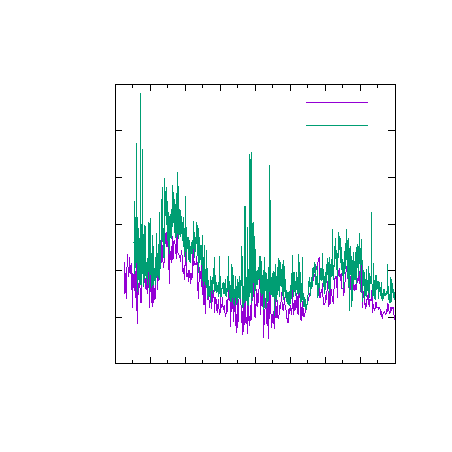
\includegraphics{../images/correlation_ts02}}%
    \gplfronttext
  \end{picture}%
\endgroup

  \caption{Time series of the \ch{NO} concentration during the two
    measurements on January 22 and January 25. Green depicts the
    chemiluminescence measurement, violet the DOAS measurement.}
  \label{fig:corr-ts}
\end{figure}

\begin{figure}[htbp]
  \centering
  \input{images/20160122_25_fixI0_corr}
  \caption{Correlation plot between our DOAS instrument and a
    chemiluminescence monitor (CLD). Each data point depicts a
    \SI{30}{\minute} average.}
  \label{fig:cld-corr}
\end{figure}
\todo{remove fit formula}

There are two avenues we took in an attempt to understand these
findings. Both of them follow arguments already layed out in
Section~\ref{sec:switch}. The first consists in the observation, that
we used the \ch{NO} calibration gas container to calibrate the
chemiluminescence display (cld). If some of the \ch{NO} had been converted
to \ch{NO2}, we would have an error in the chemiluminescence
calibration, which would lead to lower cld results. Using the above
mentioned results, we can compute that we have about \SI{420}{ppb}
\ch{NO2} in the container, if all of it stemmed from \ch{NO} this
would introduce an error of about \SI{5}{\percent} (the calibration
concentration given was $c = \SI{8.177}{ppm}$). This is not enough to
explain the descripancy. Together with the fact that we cannot
explain, how the transition from \ch{NO} to \ch{NO2} could occur, we
discard this approach.

The second avenue we took, was to look at the purge
time. Section~\ref{sec:switch} suggests that \SI{30}{\second} purge
time is not enough when the Ozone switch is turned off, as we observed
a tail in the falling flank with a natural timescale of about
\SI{146}{\second}. We were not aware of this tail when we performed
the measurements, so we tried to remedy its effects afterwards.


%%% Local Variables:
%%% mode: latex
%%% TeX-master: "../Bachelor"
%%% End:
